%%%%%%%%%%%%%%%%%%%%%%%%%%%%%%%%%%%%%%%%%%%%%%%%%%%%%%%%%%%%%%%%%%%%%%%%%%%%%%%%%%%%%%%%%%%%%%%%%%%
%%%%%%%%%%%%%%%%%%%%%%%%%%%%%%%%%%%%%%%%%%%%%%%%%%%%%%%%%%%%%%%%%%%%%%%%%%%%%%%%%%%%%%%%%%%%%%%%%%%
%%%%%%%%%%%%%%%%%%%%%%%%%%%%%%%%%%%%%%%%%%%%%%%%%%%%%%%%%%%%%%%%%%%%%%%%%%%%%%%%%%%%%%%%%%%%%%%%%%%

\chapter{Espectro evolutivo}

En esta sección se introduce el \textit{espectro evolutivo}, una generalización del espectro de 
potencias para procesos no-estacionarios cuya estructura cambia lentamente en el tiempo.
%
Esta definición en particular fue presentada por Maurice Priestley en 1965 \cite{Priestley65}; la
información del presente capítulo puede revisarse con mayor detalle en su libro \textit{"Spectral
Analysis and Time Series"} \cite{Priestley81}, particularmente en el capítulo 11.

%Las secciones \ref{sec:frecuencias2}, ..., pueden verse como preliminares de este capítulo y pueden
%omitirse en una primera lectura, pues lidian con detalles sobre diferentes posibilidades para 
%generalización el espectro.

Es importante mencionar que la sección \ref{sec:espectro} representa la parte central de este
capítulo, describiendo un objeto matemático bien definido que lidia con un problema que roza la 
vaguedad; es por ello que viene acompañado de una discusión que podría ser omitida dentro del 
contexto global del trabajo, pero que tiene repercusiones importantes en el uso práctico del 
espectro evolutivo.
%
Por ejemplo, en la sección \ref{sec:estimacion} se discute sobre las condiciones bajo las cuales es 
\textit{posible} estimar el espectro evolutivo del proceso, mientras que la sección 
\ref{sec:doble_ventana} parte de tales condiciones para describir cómo efectuar la estimación.

Finalmente, en la sección \ref{sec:psr} se describe una aplicación aparentemente menor del espectro 
evolutivo, pero que constituye una parte central en el presente trabajo: la detección de 
estacionariedad débil a partir del espectro evolutivo.

%%%%%%%%%%%%%%%%%%%%%%%%%%%%%%%%%%%%%%%%%%%%%%%%%%%%%%%%%%%%%%%%%%%%%%%%%%%%%%%%%%%%%%%%%%%%%%%%%%%
%%%%%%%%%%%%%%%%%%%%%%%%%%%%%%%%%%%%%%%%%%%%%%%%%%%%%%%%%%%%%%%%%%%%%%%%%%%%%%%%%%%%%%%%%%%%%%%%%%%

\section{Definición del espectro evolutivo}
\label{sec:espectro}

Considérese un proceso estocástico a tiempo continuo \xtin{\R} que, por simplicidad, tiene media 
cero y varianza finita en todo momento, es decir
\begin{equation*}
\E{X(t)} = 0 \text{  ,  } \Var{X^{2}(t)} < \infty
\end{equation*}

Se define el \textit{núcleo de covarianza} para el proceso como
\begin{equation}
R(s,t) := \E{\overline{X(t)}X(s)}
\end{equation}

Conviene recordar el caso de un proceso estacionario, en el cual el núcleo de covarianza $R(t,s)$ 
puede verse como función de la variable $\abso{t-s}$, y en virtud del teorema de Winer-Khintchine 
acepta una representación de la forma
%
\begin{equation}
R(s,t) = \intR e^{i \omega (t-s)} dH(\omega)
\label{s6:kernel}
\end{equation}
%
donde $H$ es el espectro integrado del proceso y tiene las propiedades de una función de 
distribución sobre $\R$.
%
Como consecuencia, \xtin{\R} admite una representación de la forma
\begin{equation}
X(t) = \intR e^{i\omega t} dZ(\omega)
\end{equation}
%
donde $Z$ es un proceso estocástico que satisface
\begin{equation}
\Cov{dZ(\omega_1),dZ(\omega_2)} = 
\begin{cases}
dH(\omega_1) &, \text{si } \omega_1 = \omega_2 \\
0 &, \text{otro caso}
\end{cases}
\end{equation}

En general, se espera tener una generalización que conserve las propiedades anteriores. Con vista
a la ecuación \ref{s6:kernel}, puede restringirse la atención a procesos no-estacionarios que
acepten una representación de la forma
\begin{equation}
R(s,t) = \intR \overline{\phi(\omega;s)}\phi(\omega;t) d\mu(\omega)
\label{s6:erre}
\end{equation}
%
Para alguna medida $\mu$ definida en $\R$ y alguna familia de funciones 
$\ef = \left\{ \phi: \R \times \mathcal{T} \rightarrow \C \right\}$; debido a la interpretación que 
se le va a dar a este tipo de funciones, la variable $t\in \ef$ será referida como un índice.
%
Una condición a satisfacer es que $\Var{X^{2}(t)} = R(t,t) < \infty$, para lo cual cada 
$\phi \in \ef$ debe ser cuadrado integrable con respecto a $\mu$, es decir
\begin{equation}
\intR \phi^{2}(\omega;t) d\mu(\omega) < \infty
\end{equation}

Se puede demostrar t(4.11.12) que bajo estas condiciones el proceso \xt acepta una representación de la forma 
\begin{equation}
X(t) = \intR \phi(\omega;t) dZ(\omega)
\label{s6:representacion}
\end{equation}
donde el proceso $Z$ satisface que
\begin{equation}
\Cov{dZ(\omega_1),dZ(\omega_2)} = 
\begin{cases}
\mu(\omega_1) &, \text{si } \omega_1 = \omega_2 \\
0 &, \text{otro caso}
\end{cases}
\end{equation}


Se puede demostrar p(parzen 1959) que si un proceso admite una representación de la forma \ref{s6:representacion} para alguna familia de funciones $\ef$, entonces tiene admite múltiples
representaciones usando diferentes familias de funciones.
%
%Para poder dar a estas representaciones la interpretación de espectro, conviene usar una familia de
%funciones que conserven algunas propiedades de los senos y cosenos.
%

Para dar a estas representaciones la interpretación de espectro, conviene usar una familia de funciones que conserve algunas propiedades de los senos y cosenos; por ejemplo, las funciones oscilatorias

\begin{definicion}
Una función $\phi: \R \rightarrow \C$ se dice \textbf{oscilatoria} si admite una representación de la forma
\begin{equation}
\phi(t) = A(t) e^{i \omega t} 
\end{equation}
donde $A$ es de la forma
\begin{equation}
A(t) = \intR e^{i \omega t} dK(\omega)
\end{equation}
y donde $\abso{dK(\omega)}$ tiene un único máximo global en $\omega = 0$
\label{oscilatorio}
\end{definicion}

Si una función $\phi$ es oscilatoria como en la definición \ref{oscilatorio}, entonces puede entenderse como una función senoidal \textit{modulada} por una función $A$; no se permite que la función $A$ sea predominantemente periódica.

Como se mencionó, las expresiones \ref{s6:erre} y \ref{s6:representacion} pueden ser interpretadas como espectro si se usa una familia $\ef$ de funciones oscilatorias.

\begin{align}
R(s,t) &= \intR \overline{A(\omega; s)} A(\omega; t) e^{i\omega (t-s)} d\mu(\omega) \\
X(t) &= \intR A(\omega; t) e^{i \omega t} dZ(\omega)
\end{align}


\begin{definicion}
Sea \xt un proceso oscilatorio y $\ef$ una familia de funciones oscilatorias de la forma
$\phi(\omega;t) = A(\omega;t) e^{i \omega t}$. 
Sea $\mu$ tal que ...
Se define al \textbf{espectro evolutivo} del proceso respecto a la familia $\ef$ como
\begin{equation}
dH(t,\omega) := \abso{A(\omega;t)}^{2} d\mu(\omega)
\end{equation}
\label{def:oscilatorio}
\end{definicion}

%%%%%%%%%%%%%%%%%%%%%%%%%%%%%%%%%%%%%%%%%%%%%%%%%%%%%%%%%%%%%%%%%%%%%%%%%%%%%%%%%%%%%%%%%%%%%%%%%%%
%%%%%%%%%%%%%%%%%%%%%%%%%%%%%%%%%%%%%%%%%%%%%%%%%%%%%%%%%%%%%%%%%%%%%%%%%%%%%%%%%%%%%%%%%%%%%%%%%%%

\section{Estimación del espectro evolutivo}
\label{sec:estimacion}

En el capítulo anterior se mostró un estimador consistente para el espectro de potencias de un proceso estacionario; dicho estimador usaba la transformada de Fourier discreta, \textit{suavizada} por un filtro lineal (también referido como función ventana).
%
El objetivo de esta sección es aclarar algunos teoremas que permitan usar una técnica similar, la cual requiere imponer algunas condiciones más fuertes que ser oscilatorios.

\subsection{Filtros lineales}

Sea \xt un proceso oscilatorio, no necesariamente estacionario, y sea $g\in \lldos$; se construye al proceso $\{Y(t)\}_{t\in \mathcal{T}}$ como\footnote{En el texto de Priestley se considera un filtro de la forma $Y(t) = \intR g(u) X(t-u) e^{-i \omega_0 (t-u)} du$ para algún $\omega_0$ constante. 
Por simplicidad se considera únicamente el caso $\omega_0=0$}
\begin{equation}
Y(t) = \intR g(u) X(t-u) du
\end{equation}

Entonces puede escribirse 
\begin{equation}
Y(t) = \intR \Gamma_t(\omega) e^{i \omega t} dZ(\omega) 
\label{se6:filtrado}
\end{equation}
donde $\Gamma_\bullet$ es la \textbf{función de transferencia generalizada} para $g$ con respecto a la familia $\ef$, y que es definida como
\begin{equation}
\Gamma_t (\omega) := \intR g(u) A(\omega; t-u) e^{i \omega u} du
\label{se6:trans_general}
\end{equation}

%En general no puede garantizarse que la expresión en \ref{se6:filtrado} satisfaga las propiedades de un espectro evolutivo; si se escribe
%\begin{equation*}
%\Gamma_t(\omega) = \intR e^{i \omega t} dK(\omega)
%\end{equation*}
%no siempre se cumple que $\abso{dK}$ tiene un único máximo global en 0.

Un caso particular muy interesante ocurre cuando $A$, como función de $\omega$, varía lentamente en comparación de $g$, la cual decae rápidamente a 0; en tal caso podría decirse que $\Gamma_\bullet \approx \Gamma$


\begin{definicion}
Una familia de funciones $\ef$ se dice \textbf{semi-estacionaria} si, para todo $\omega \in \R$, se cumple que
\begin{equation}
\intR \abso{\omega} \abso{dK(\omega)} < \infty
\end{equation}
En cuyo caso se define su \textbf{ancho característico}
\begin{equation}
B_\ef := \left[ \sup_\omega \intR \abso{\omega} \abso{dK(\omega)} \right]^{-1}
\end{equation}
\end{definicion}

\begin{definicion}
Un proceso \xt se dice \textbf{semi-estacionario} si admite una representación de la forma \ref{s6:representacion} para alguna familia semi-estacionaria
\end{definicion}

%\begin{definicion}
%Sea \xt un proceso semi-estacioario, y sea $\mathcal{C}$ la clase de las familias semi-estacionarias con las cuales el proceso admite una representación de la forma [?].
%Se define el \textbf{ancho de banda característico} de \xt como 
%\begin{equation}
%B_X := \sup_{\ef \in \mathcal{C}} B_\ef
%\end{equation}
%\end{definicion}

\begin{definicion}
Se dice que una función $u$ es 
\textbf{pseudo-$\boldsymbol{\delta}$ de orden $\boldsymbol{\varepsilon}$} con respecto a la función $v$ si, para cualquier $k$ existe un $\varepsilon << 1$ tal que 
\begin{equation}
\abso{\intR u(x) v(x+k) dx  -  v(k)\intR u(x)} < \varepsilon
\end{equation}
\end{definicion}


De manera similar, se define el \textbf{ancho de banda} para $g$ como 
\begin{equation}
B_g := \intR \abso{u} \abso{g(u)} du
\end{equation}

Supóngase que $g$ está normalizada de modo que
\begin{equation}
2 \pi \intR \abso{g(u)}^{2} du = \intR \abso{\Gamma(\omega)} d\omega = 1
\label{s6:norm_g}
\end{equation}
con $\Gamma$ la función de respuesta para $g$.

\begin{teorema}
Sea $\ef$ una familia semi-estacionaria con ancho de banda característico $B_\ef$, y sea $g$ una función normalizada como en \ref{s6:norm_g} y cuyo ancho de banda es $B_g$. Entonces, para cualesquiera $t, \omega \in \R$ se cumple que $e^{i \omega t} dK(\omega)$ es una función pseudo-$\delta$ de orden $\nicefrac{B_g}{B_\ef}$ con respecto a $g$
\label{teo:s6:lema}
\end{teorema}
\begin{proof}
Suponiendo que $\Gamma$ sea una vez derivable, su expansión de Taylor alrededor de $k$ es
\begin{equation*}
\intR e^{i\theta t} \Gamma(\theta + k) dK(\omega)
= \Gamma(k) \intR e^{i \theta t} dK(\omega) + 
\intR e^{i \theta t} \theta \Gamma\prima(k + \nu) dK(\omega)
\end{equation*}
para algún $\nu \in (0,\theta)$. Respecto al segundo sumando, puede observarse que
\begin{align*}
\intR e^{i \theta t} \theta \Gamma\prima(k + \nu) dK(\omega)
&\leq
\abso{ \intR e^{i \theta t} \theta \Gamma\prima(k + \nu) dK(\omega)} \\
&\leq
\intR \abso{ \theta} \abso{ \Gamma\prima(k + \nu)} \abso{ dK(\omega)} \\
&\leq
\intR \abso{ \theta} \left[ \sup_\omega \abso{ \Gamma\prima(\omega)} \right] \abso{ dK(\omega)} \\
&\leq
\left[ \sup_\omega \abso{ \Gamma\prima(\omega)} \right]
\left[ \sup_\omega
\intR \abso{ \theta} \abso{ dK(\omega)} \right]
\end{align*}
Usando la conexión entre $g$ y $\Gamma$
\begin{align*}
\Gamma\prima(\omega) 
&= \frac{d}{d\omega} \left( \intR e^{i \omega u} g(u) du \right) \\
&= \intR \left( \frac{d}{d\omega} e^{i \omega u} g(u) \right) du \\
&= i \intR u e^{i \omega u} g(u) du \\
\end{align*}
Luego entonces
\begin{align*}
\intR e^{i \theta t} \theta \Gamma\prima(k + \nu) dK(\omega)
&\leq
\left[ \sup_\omega \abso{ \Gamma\prima(\omega)} \right] 
\left[ \sup_\omega
\intR \abso{ \theta} \abso{ dK(\omega)} \right] \\
&\leq 
\left[ \sup_\omega \abso{ \intR i u e^{i \omega u} g(u) du } \right] 
B_\ef^{-1} \\
&\leq 
B_\ef^{-1}
\left[ \sup_\omega \intR \abso{ u } \abso{ g(u)} du \right] \\
&\leq
B_\ef^{-1} B_g
\end{align*}
\end{proof}

Con el teorema anterior a la mano se puede declarar formalmente la idea de que $A$ varía más lentamente que $g$

\begin{teorema}
Sea $\ef$ una familia semi-estacionaria con ancho de banda característico $B_\ef$, sea $\varepsilon >0$ arbitrario, y sea $g$ un filtro normalizado como en \ref{s6:norm_g} y cuya función de transferencia generalizada con respecto a $\ef$ es $\Gamma_\bullet$. 
%
Si $g$ es elegida de tal modo que $\nicefrac{B_g}{B_\ef} < \varepsilon$, entonces para cualesquiera $t, \omega$ se cumple que
\begin{equation}
\abso{\Gamma_t(\omega)- A(\omega; t)\Gamma(\omega)} < \varepsilon
\end{equation}
\label{teo:aprox_gamma} 
\end{teorema}

\begin{proof}
Por la mera definición de $\Gamma_\bullet$ (expresión \ref{se6:trans_general}) se sabe que
\begin{equation*}
\Gamma_t (\omega) = \intR g(u) A(\omega; t-u) e^{i \omega u} du
\end{equation*}
Si se sustituye a $A$ en términos de $dK$ (ver definición \ref{def:oscilatorio})
\begin{align*}
\Gamma_t (\omega) &= \intR g(u) A(\omega; t-u) e^{i \omega u} du \\
&= 
\intR g(u) \left[ \intR e^{i \theta (t-u)} dK(\theta) \right] e^{i \omega u} du \\
&=
\intR \intR g(u) e^{i \theta t} e^{i (\omega- \theta) u} dK(\theta) du \\
&=
\intR e^{i \theta t} \left[ \intR g(u) e^{i (\omega- \theta) u} du \right] dK(\theta) \\
&=
\intR e^{i \theta t} \Gamma(\omega - \theta) dK(\theta) \\
\end{align*}
Usando el lema \ref{teo:s6:lema} junto al hecho que $\nicefrac{B_g}{B_\ef} < \varepsilon$, se puede escribir que
\begin{align*}
\varepsilon 
&> 
\abso{\intR e^{i \theta t} \Gamma(\omega - \theta) dK(\theta) - 
\Gamma(\omega) \intR e^{i \theta t} dK(\theta) } \\
&=
\abso{\Gamma_t (\omega) - 
\Gamma(\omega) \intR e^{i \theta t} dK(\theta) } \\
&=
\abso{\Gamma_t (\omega) - 
\Gamma(\omega) A(\omega; t) }
\end{align*}
En el último renglón se ha reemplazado nuevamente a $A$ en términos de $dK	$
\end{proof}

\begin{teorema}
Sea \xt un proceso semi-estacionario con ancho de banda característico $B_X$, sea $g$ un filtro normalizado como en \ref{s6:norm_g} y cuyo ancho de banda es $B_g$ y cuya función de respuesta es $\Gamma$. 
%
Sea $\{Y(t)\}_{t\in \mathcal{T}}$ un proceso definido como \ref{se6:filtrado}.

Sea $\efstar$ una familia semi-estacionaria cuyo ancho de banda característico es $B_X$ o es muy parecido a $B_X$ (lo cual es posible por cómo se definió $B_X$).
Se cumple que
\begin{equation}
\E{\abso{Y(t)}^{2}} = \intR \abso{\Gamma(\omega)}^{2} dH^{*}(\omega; t) + \orden{\epsilon}
\end{equation}
donde $H^{*}$ es el espectro integrado respecto a la familia $\efstar$ y $\orden{\epsilon}$ es un término que puede hacerse arbitrariamente pequeño si $B_g$ es suficientemente pequeño respecto a $B_X$
\label{teo:aprox_orden}
\end{teorema}

\begin{proof}
Usando la expresión \ref{se6:filtrado} para este caso particular, puede escribirse
\begin{equation}
Y(t) = \intR \Gamma_t^{*} (\omega; t) A^{*}(\omega; t) e^{i \omega t} dZ^{*}(\omega)
\end{equation}
donde $\omega_\bullet^{*}$, $A^{*}$ y $Z^{*}$ están definidos respecto a la familia $\efstar$.
Nótese que, debido a que los $dZ$'s son ortogonales
\begin{align*}
\E{\abso{Y(t)}^{2}} 
&= 
\E{
\overline{\intR \Gamma_t^{*} (\omega; t) e^{i \omega t} dZ^{*}(\omega)}
\intR \Gamma_t^{*} (\omega; t) e^{i \omega t} dZ^{*}(\omega) }\\
&= ... \\
&= \intR \abso{\Gamma_t^{*} (\omega; t)}^{2} d\mu^{*}(\omega)
\end{align*}

Si se elige a $g$ de modo que $\frac{B_g}{B_X} < \varepsilon$, en virtud del teorema \ref{teo:aprox_gamma} puede escribirse
\begin{equation}
\Gamma_t^{*}(\omega; t) = A^{*}(\omega; t) \Gamma(\omega) + R(\omega; t)
\end{equation}
con $\abso{R(\omega,t)} < \varepsilon$. Luego entonces
\begin{align*}
\E{\abso{Y(t)}^{2}} 
&= 
\intR \abso{\Gamma_t^{*} (\omega; t)}^{2} d\mu^{*}(\omega) \\
&= 
\intR \abso{A^{*}(\omega; t) \Gamma(\omega) + R(\omega; t)}^{2} d\mu^{*}(\omega) \\
&= 
\intR \abso{A^{*}(\omega; t) \Gamma(\omega)}^{2} d\mu^{*}(\omega) +\\
&\pheq
\intR \overline{A^{*}(\omega; t) \Gamma(\omega)} R(\omega; t) d\mu^{*}(\omega) +\\
&\pheq
\intR A^{*}(\omega; t) \Gamma(\omega) \overline{ R(\omega; t)} d\mu^{*}(\omega) +\\
&\pheq
\intR \abso{R(\omega; t)}^{2} d\mu^{*}(\omega) 
\end{align*}

El cuarto sumando satisface claramente que
\begin{equation}
\intR \abso{R(\omega; t)}^{2} d\mu^{*}(\omega)  < \varepsilon^{2} \intR d\mu^{*}(\omega) 
= \orden{\varepsilon^{2}}
\end{equation}

Respecto al segundo sumando, nótese que 
\begin{align*}
\intR \overline{A^{*}(\omega; t) \Gamma(\omega)} R(\omega; t) d\mu^{*}(\omega)
&< \intR \abso{A^{*}(\omega; t)} \abso{ \Gamma(\omega)} \abso{R(\omega; t)} d\mu^{*}(\omega) \\
&< \varepsilon \intR \abso{A^{*}(\omega; t)}\abso{ \Gamma(\omega)} d\mu^{*}(\omega)
\end{align*}
Una cota similar puede hallarse para el tercer sumando.
Falta demostrar que la cota permanece finita cuando $B_g \rightarrow 0$, lo cual debería lograrse definicendo el conjunto
\begin{equation}
\Omega = \left\{ \omega \in \R | \abso{\Gamma(\omega)} \abso{A^{*}(\omega; t)} \leq 1 \right\} 
\end{equation}
y luego, claramente
\begin{equation}
\intR \abso{A^{*}(\omega; t)}\abso{ \Gamma(\omega)} d\mu^{*}(\omega) = 
\int_\Omega \mu^{*}(\omega) + 
\int_{\Omega^{C}} \abso{A^{*}(\omega; t)}\abso{ \Gamma(\omega)} d\mu^{*}(\omega)
\end{equation}
el primer sumando es clarametne finito y no depende de $g$, mientras que el segundo debería ser finito [?] ya que $\Gamma$ está normalizada.
\end{proof}

%%%%%%%%%%%%%%%%%%%%%%%%%%%%%%%%%%%%%%%%%%%%%%%%%%%%%%%%%%%%%%%%%%%%%%%%%%%%%%%%%%%%%%%%%%%%%%%%%%%
%%%%%%%%%%%%%%%%%%%%%%%%%%%%%%%%%%%%%%%%%%%%%%%%%%%%%%%%%%%%%%%%%%%%%%%%%%%%%%%%%%%%%%%%%%%%%%%%%%%

\section{Estimador de doble ventana}
\label{sec:doble_ventana}

Para esta sección se considera un proceso a tiempo continuo \xtin{\R} y una muestra del mismo de longitud $T$ (o equivalentemente un proceso \xtin{[0,T]}), suficientemente larga. El objetivo en esta sección es construir un estimador para el espectro evolutivo $dH(\omega; t)$.
%
Por simplicidad, se supondrá que la medida $\mu$ es absolutamente continua respecto a la medida de Lebesgue, y entonces puede escribirse
\begin{equation}
h(\omega,t) := dH(\omega; t)
\end{equation}

Para efectuar la estimación del espectro se hará uso del teorema \ref{teo:aprox_gamma}, para lo cual se necesita un filtro $g$ normalizado según \ref{s6:norm_g} y cuyo anho de banda, $B_g$, satisface
\begin{equation}
B_g << B_X << T
\label{s6:anchos_banda}
\end{equation}

Se construye entonces a $U$, una versión filtrada de $X$ usando a $g$
\begin{equation}
U(t) = \int_{t-T}^{t} g(u) X(t-u) du
\end{equation}

Bajo la condición \ref{s6:anchos_banda}, la integral que define a $U$ puede extenderse a todo $\R$ sin cambiar mucho su valor (excepto cerca de 0 y $T$), e incluso se llega a ser exacta si $g$ es 0 fuera de un intervalo pequeño alrededor de 0. Entonces, en virtud del teorema \ref{teo:aprox_orden}
aplica de manera aproximada, y entonces se cumple que
\begin{equation}
\E{\abso{U(\omega; t)}^{2}} = \intR \abso{\Gamma(\omega)}^{2} h(\omega, t)d\omega + \orden{\nicefrac{B_g}{B_X}}
\end{equation}


\begin{proposicion}
Dadas las condiciones, y si \xt es un proceso normal cuyo que admite un espectro evolutivo uniformemente continuo, se tiene que
\begin{equation}
\Var{\abso{U(\omega;t)}^{2}} \approx \left[ \intR \abso{\Gamma(\omega)}^{2} h(\omega, t)d\omega \right]^{2}
\end{equation}
\end{proposicion}

La demostración al teorema anterior puede ahllarse en el artículo de Maurice Priestley \textit{Design Relations for Non-Stationary Processes} \cite{Priestley66}, sección 3.

%\begin{proof}
%En general, puede escribirse para $t,s \in \mathcal{T}$, $\omega, \lambda \in \R$
%\begin{align*}
%\Cov{\abso{U(\omega;t)}^{2},\abso{U(\lambda;s)}^{2}} &=
%\E{\abso{U(\omega;t)}^{2},\abso{U(\lambda;s)}^{2}} \\
%&=
%\int \int \int \int_{R^{4}} g(u) g(v) g(w) g(z) e^{i u \omega} e^{i v \omega} e^{i w \lambda} e^{i z \lambda} \\
%&\pheq \times
%\E{{X(t-u)} {X(t-v)} {X(s-w)} {X(s-z)}}
%du dv dw dz 
%\end{align*}
%Si \xt es normal, entonces
%\begin{align*}
%\E{X(t-u) {X(t-v)} {X(t-w)} X(t-z)} &=
%R(t-u,t-v)R(s-w,s-z) \\
%&\pheq + R(t-u,s-z)R(t-v,s-w) \\
%&\pheq + R(t-u,s-w)R(t-v,s-z)
%\end{align*}
%donde
%\begin{equation}
%R(p,q) = \intR e^{i \omega (p-q)} A(\omega; p)\overline{A(\omega; q)} d\mu(\omega) 
%\end{equation}
%Así entonces, puede escribirse
%\begin{align*}
%\Cov{\abso{U(\omega;t)}^{2},\abso{U(\lambda;s)}^{2}} &=
%\E{\abso{U(\omega, t)}^{2}} \E{\abso{U(\lambda, s)}^{2}} + S_1 + S_2
%\end{align*}
%donde
%\begin{align*}
%S_1 &= 
%\int \int \int \int_{\R^{4}} g(u) g(v) g(w) g(z) e^{i u \omega} e^{i v \omega} e^{i w \lambda} e^{i z \lambda} \\
%&\pheq \times \left( 
%\int \int_{\R^{2}} 
%\left[ 
%e^{-i \theta (s-z-t+u)} A(\theta; t-u) \overline{A(\theta; s-z)} 
%\right] 
%\right. \\
%&\pheq 
%\left. \vphantom{\int}
%\left[ e^{-i \phi (s-w-t+u)} A(\phi; t-v) \overline{A(\theta; s-w)} \right] d\theta d\phi
%\right) du dv dw dz
%\end{align*}
%Puede escribirse
%\begin{align*}
%S_1 &= \int \int_{\R^{2}} \Gamma(\theta+ \omega; t, \theta) \overline{\Gamma(\phi + \omega; t, \phi)}
% \Gamma(\phi+ \lambda; s, \phi) \overline{\Gamma(\theta + \lambda; s, \theta)} \\
% &\pheq \times
% \left[
% A(\theta; t) \overline{A(\phi; t)} A(\phi; s) \overline{A(\theta; t)}
% \right] d\theta d\phi
%\end{align*}
%Usando el teorema [?], si $B_g << B_X$ entonces $\Gamma(\bullet; t, \lambda) \approx \Gamma(\bullet)$, luego
%\begin{align*}
%S_1 &\approx \left[ e^{-i \theta (s-t) } A(\theta; t) \overline{A(\theta; s)} \Gamma(\theta + \omega) \Gamma(\theta + \lambda) d\theta\left] \\
%\phantom{\approx} \times
%\left[ e^{-i \phi (s-t) } A(\theta; t) \overline{A(\phi; s)} \Gamma(\phi + \omega) \Gamma(\phi + \lambda) d\phi\left] \\
%\end{align*}
%\end{proof}

Un resultado que es muy análogo a la estimación del espectro en el caso de estacionariedad.
%
Siguiendo con la analogía, este problema es resuelto al usar un filtro $w_\tau$ que satisfaga las siguientes propiedades
\begin{itemize}
\item $w_\tau(t) \geq 0$ para cualesquiera $t$, $\tau$
\item $w_\tau(t) \rightarrow 0$ cuando $\abso{t} \rightarrow \infty$, para todo $\tau$
\item $\displaystyle \intR w_\tau(t) dt = 1$ para todo $\tau$
\item $\displaystyle \intR \left( w_\tau(t) \right)^{2} dt < \infty$ para todo $\tau$
\item $\exists C \in \R$ tal que  
$\displaystyle \lim_{\tau\rightarrow\infty} \tau \intR \abso{ W_{\tau}(\lambda) }^{2} d\lambda = C$
\end{itemize}
donde $W_\tau = \intR e^{-i \lambda t} w_\tau(t) d\lambda$. Se define el segundo estimador
\begin{equation}
V(t) = \int_{T-t}^{t} w_\tau (u) \abso{U(t-u)}^{2} du
\label{estimador_doble_ventana}
\end{equation}

El supuesto sobre que $g$ decaiga lejos de 0, aplicado ahora a $w_\tau$, permite reemplazar el intervalo de integración que define a $V$ por $\R$. 

De manera sencilla puede verse que
\begin{align*}
\E{V(t)} &= 
\E{\intR w_\tau (u) \abso{U(t-u)}^{2} du} \\
&= 
\int_{T-t}^{t} w_\tau (u) \E{\abso{U(t-u)}^{2}} du \\
&=
\intR w_\tau (u) \left[
\intR \abso{\Gamma(\omega)}^{2} h(\omega, t-u)d\omega + \orden{\nicefrac{B_g}{B_X}} \right] du \\
&=
\intR \intR w_\tau (u) \abso{\Gamma(\omega)}^{2} h(\omega, t-u)d\omega du +
\orden{\nicefrac{B_g}{B_X}} \intR w_\tau (u) du \\
&=
\intR \abso{\Gamma(\omega)}^{2} \left[ \intR w_\tau (u) h(\omega, t-u) du \right] d\omega du +
\orden{\nicefrac{B_g}{B_X}} \intR w_\tau (u) du \\
&=
\intR \abso{\Gamma(\omega)}^{2} \overline{h}(\omega,t) d\omega du +
\orden{\nicefrac{B_g}{B_X}} \\
\end{align*}
donde
\begin{equation}
\overline{h}(\omega,t) = \intR w_\tau (u) h(\omega, t-u) du
\end{equation}

Es demostrado en Priestley [1966?] que
\begin{equation}
\Var{V(t)} \approx \widetilde{h}^{2}(\omega_0,t) \left[ \intR \abso{W_\tau(\omega)}^{2} d\omega \right] \left[ \intR \abso{\Gamma(\omega)}^{4} \right] (1+\delta(0,\omega_0))
\end{equation}
donde
\begin{equation}
\widetilde{h}^{2} = \frac{\intR h^{2}(\omega_0,t) \left(w_\tau(u)\right)^{2}}{\intR \left(w_\tau(u)\right) du}
\end{equation}

Aún más, si se usa la propiedad de en el límite de $\tau W_\tau$ se puede escribir
\begin{equation}
\Var{V(t)} \approx 
\widetilde{h}^{2}(\omega_0,t) \frac{C}{\tau} \left[ \intR \abso{\Gamma(\omega)}^{4} \right] (1+\delta(0,\omega_0))
\end{equation}

Una aproximación muy similar 
puede hacerse respecto al segundo término, de modo que $\widetilde{h}\approx h$ y 
$\overline{h}^{2}\approx h^{2}$.
Tales aproximaciones serán mejores en tanto las ventanas $w_{\tau}$ y $W_{\tau}$ sean más 
cercanas a funciones tipo \dirac.
Dicho esto, se pueden hacer las siguientes aproximaciones, un poco más arriesgadas:
\begin{itemize}
\item $\displaystyle \E{\est{h}(t,\omega)} \approx h(t,\omega)$
\item $\displaystyle \Var{\est{h}(t,\omega)} \approx 
\frac{C}{\tau} h^{2}(t,\omega) \intR \abso{\Gamma_\kappa (\theta)}^{4} d\theta$
\end{itemize}

%%%%%%%%%%%%%%%%%%%%%%%%%%%%%%%%%%%%%%%%%%%%%%%%%%%%%%%%%%%%%%%%%%%%%%%%%%%%%%%%%%%%%%%%%%%%%%%%%%%
%%%%%%%%%%%%%%%%%%%%%%%%%%%%%%%%%%%%%%%%%%%%%%%%%%%%%%%%%%%%%%%%%%%%%%%%%%%%%%%%%%%%%%%%%%%%%%%%%%%

\section{Prueba de Priestley-Subba Rao}
\label{sec:psr}

La prueba de estacionariedad propuesta por Priestley y Subba Rao \cite{Priestley69} consiste en 
probar la hipótesis de que el espectro evolutivo efectivamente cambia en el tiempo. 
%
El proceso consiste en \textit{calcular} el logaritmo del espectro evolutivo para algunos tiempos y 
frecuencias puntuales, para lo cual se usa el estimador de doble ventana, y posteriormente usar un
análisis ANOVA para verificar si dichas cantidades tienen el mismo valor esperado --recordando que
el estimador de doble ventana es asintóticamente consistente.

Sea \xt un proceso semi-estacionario y sea \xtd un conjunto de observacion, cuya frecuencia de 
muestreo es $\Delta_t=1$ por simplicidad.
%
Usando estos datos se construye el estimador de doble ventana, $\widehat{h}$; para ello se eligen 
como parámetros las funciones $g_\kappa$ y $w_\tau$, que dependen a su vez de los parámetros 
$\kappa$ y $\tau$, y por consecuencia a sus respectivas tr. de Fourier $\Gamma_\kappa$ y $W_\tau$.
%
Bajo las condiciones descritas en la sección anterior, se satisface que
%
\begin{align*}
\E{\widehat{h}(t,\omega)} &\approx h(t,\omega) \\
\Var{\widehat{h}(t,\omega)} &\approx 
\frac{C}{N} h^{2}(t,\omega) \intR \abso{\Gamma^{4}(\theta)} d\theta
\end{align*}
%
donde $\displaystyle C = \lim_{T\rightarrow \infty} T \intR \abso{W_T(\lambda)} d\lambda$.
%
Como es habitual en el estudio del espectro de potencias, se propone la cantidad 
\begin{equation}
Y(t,\omega) = \log\left(\widehat{h}(t,\omega)\right)
\end{equation}
que, por ser $\log$ una función inversible y derivable, cumple que
%
\begin{align*}
\E{Y(t,\omega)} &\approx \log\left(h(t,\omega)\right) \\
\Var{Y(t,\omega)} &\approx 
\frac{C}{T} \intR \abso{\Gamma_\kappa(\theta)}^{4} d\theta \\
\end{align*}

Cabe destacar que la varianza de $Y$ no es independiente de $h$ en el sentido formal, sino que 
sólo es \textit{aproximadamente independiente} pues depende en mayor medida de la forma de 
$\widehat{h}$ que del mismo $h$.
%
Esto era de esperarse, ya que el estimador de doble ventana fue diseñado para exagerar el 
\textit{peso} de la información local. 
%
En otra dirección, la independencia aproximada sugiere que $Y$ puede escribirse como

\begin{equation}
Y(t,\omega) = \log\left(h(t,\omega) \right) + \varepsilon(t,\omega)
\label{ye}
\end{equation}
%la cual \textit{hereda} las características
%\begin{align*}
%\E{\varepsilon(t,\omega)} &\approx 0 \\
%\Var{\varepsilon(t,\omega)} 
%&\approx \frac{C}{T} \intR \abso{\Gamma_\kappa(\theta)}^{4} d\theta
%\end{align*}

El que la varianza de $Y$ sea aproximadamente constante en todos los tiempos y frecuencias lo hace 
una excelente elección para verificar que el espectro evolutivo es constante en el tiempo.
%
Dos problemas respecto a la expresión \ref{ye} son (1) la covarianza de $\varepsilon$ entre
tiempos y frecuencias y (2) computacionalmente sólo es posible evaluar a $Y$ sobre una malla
de puntos en tiempo y frecuencia.

Sea una malla de puntos en el tiempo y las frecuencias, equiespaciado en el tiempo con distancia 
$\delta_t$ y en las frecuencias con distancia $\delta_\omega$.
%$\left\{ (t_i,\omega_j) \in \mathcal{T} \times [-\pi,\pi] | i = 1,\dots,I ; j=1,\dots,J \right\}$
Es demostrado en \cite{Priestley66} que si $\delta_\omega$ o $\delta_t$ son suficientemente grandes
como para que se cumpla alguna de las condiciones en \ref{separacion}, entonces los valores de $Y$
sobre la cuadrícula son aproximadamente no-correlacionados.

\begin{equation}
\left.
\begin{aligned}
\intR \abso{\Gamma_\kappa(\theta)}^{2}\abso{\Gamma_\kappa(\theta+\delta_\omega)}^{2} d\theta 
&\approx 0 \\
\frac{1}{\delta_t} \intR \abso{t} \abso{w_\tau (t)} dt &\approx 0
\end{aligned}
\right\rbrace
\Rightarrow
\Cov{Y(t,\omega),Y(t,\omega_0)} \approx 0
\label{separacion}
\end{equation}

Así entonces, sea
$\left\{ (t_i,\omega_j) \in \mathcal{T} \times [-\pi,\pi] | i = 1,\dots,I ; j=1,\dots,J \right\}$
la cuadrícula descrita, con $\delta_t= \abso{t_i - t_{i+1}}$ y 
$\delta_\omega = \abso{\omega_j-\omega_{j+1}}$. 
%
Se define el estimador
\begin{equation}
Y_{i,j} = \log\left(\widehat{h}(t_i,\omega_j)\right)
\end{equation}
%
el cual tiene las siguientes propiedades
%
\begin{align*}
Y_{i,j} &\approx \log\left(h(t_i,\omega_j)\right) + \varepsilon_{i,j} \\
\E{\varepsilon_{i,j}} &\approx 0 \\
\Var{\varepsilon_{i,j}} &\approx
\frac{C}{T} \intR \abso{\Gamma_\kappa(\theta)}^{4} d\theta \\
\Cov{\varepsilon_{i,j},\varepsilon_{i_0,j_0}} &\approx 0 
\Leftarrow (i,j)\neq (i_0,j_0)
\end{align*}

%Si el número de puntos es \textit{suficientemente grande}, entonces aproximadamente
%$\varepsilon_{i,j} \sim N(0,\sigma^{2})$.

Una vez definido un estimador adecuado para detectar la estacionariedad débil, conviene escribir
explícitamente las condiciones para tal detección.
%
La estacionariedad débil, en términos del espectro evolutivo $h$, puede expresarse como
%
\begin{equation*}
H_{E_1} : h(t_0,\omega_j) = h(t_1,\omega_j) = \cdots = h(t_I,\omega_j)
\text{ , para } j = 1, 2, \dots , J
\end{equation*}
%
condición que puede reescribirse\footnote{$H_{E_1}$ y $H_{E_2}$ son equivalentes en cuanto a la
decisión que producen} en términos de $Y$, en su versión discreta
%
\begin{equation*}
H_{E_2} : \E{Y_{0,j}} = \E{Y_{1,j}} = \cdots = \E{Y_{I,j}} \text{ , para } j = 1, 2, \dots , J
\end{equation*}
%
la cual, a su vez, puede reescribirse como
\begin{equation*}
H_{E_3} : \E{\varepsilon_{0,j}} = \E{\varepsilon_{1,j}} = \cdots =
\E{\varepsilon_{I,j}} \text{ , para } j = 1, 2, \dots , J
\end{equation*}

Sin embargo, la condición $H_{E_3}$ es una consecuencia directa de las propiedades de $Y$ si
$H_{E_2}$ es cierta; este \textit{juego} de equivalencias pierde consistencia si resulta que
$H_{E_3}$ fuera rechazada, lo cual implicaría en una contradicción.

El objetivo de la prueba puede fijarse en verificar efectivamente ocurre la contradicción
referida, en cuyo caso se podrá concluir que el proceso \textbf{no} es débilmente estacionario.
%
Con base a la forma de $H_{E_2}$, la prueba puede formularse en términos de un análisis ANOVA de dos
factores, el cual parte de un modelo general
%
\begin{equation*}
H_0 : Y_{i,j} = \mu + \alpha_i + \beta_j + \gamma_{i,j} + \varepsilon_{i,j}
\end{equation*}
%
donde $\varepsilon$ es como se definió anteriormente. 
%
Dentro del contexto, las cantidades involucradas pueden interpretarse como
\begin{description}
\item[$\mu$] Promedio de $h$ sobre tiempo y frecuencia
\item[$\alpha$] Efecto al variar el tiempo
\item[$\beta$] Efecto al variar la frecuencia
\item[$\gamma$] Efecto no lineal de tiempo y frecuencia (\textit{interacción})
\end{description}

La diferencia entre $\gamma$ y $\varepsilon$ consiste en que se conocen (por diseño) la media y 
varianza de $\varepsilon$, y se espera que siga una distribución normal si se cuentan con 
suficientes puntos; en contraparte, no se ha supuesto nada sobre $\gamma$.

Ahora bien, la hipótesis $H_{E_2}$ puede reescribirse para contrastarse contra $H_0$ como
%
\begin{equation*}
H_A : \hspace{1em} Y_{i,j} = \mu + \alpha_i + \varepsilon_{i,j}
\end{equation*}

Por simplicidad, conviene considerar un paso intermedio
\begin{equation*}
H_{\text{inter}} : Y_{i,j} = \mu + \alpha_i + \beta_j + \varepsilon_{i,j}
\end{equation*}

Como es usual con los ANOVA, se definen las sumas de cuadrados dentro de los grupos y entre los
grupos (cuadro \ref{cantidades_psr}), las cuales siguen distribuciones $\chi^{2}$.
%
Al probar $H_0$ contra $H_{\text{inter}}$ se usa el estadístico de prueba 
$\nicefrac{S_{I+R}}{\sigma^{2}}$, mientras que al probar $H_{\text{inter}}$ contra $H_A$ se usa
$\nicefrac{S_T}{\sigma^{2}} = 0$.

\begin{table}
\caption{Estadísticos involucrados en la prueba PSR}
\centering
\bordes{1.1}
\begin{tabular}{lll}
\toprule
Descripción & Estadístico & {Gr. de libertad} \\
\midrule
Efecto tiempo &
$S_T =J \sum_{i=1}^{I} \left( Y_{i,\bullet} - Y_{\bullet,\bullet} \right)^{2}$ 
& $I-1$ \\
Efecto frecuencia &
$S_F = I \sum_{j=1}^{J} \left( Y_{\bullet,j} - Y_{\bullet,\bullet} \right)^{2}$ 
& $J-1$ \\
Interacción &
$S_{I+R} = \sum_{i=1}^{I} \sum_{j=1}^{J} 
\left( Y_{i,j} - Y_{i,\bullet} - Y_{\bullet,j} + Y_{\bullet,\bullet} \right)^{2}$ 
& $(I-1)(J-1)$ \\
%\midrule
\rowcolor{gris}
Total &
$S_{0} = \sum_{i=1}^{I} \sum_{j=1}^{J} 
\left( Y_{i,j} - Y_{\bullet,\bullet} \right)^{2}$ 
& $IJ -1$ \\
\midrulec
Prom. tiempo &
$Y_{i,\bullet} = \frac{1}{J} \sum_{j=1}^{J} Y_{i,j}$ & \\
Prom. frecuencia &
$Y_{\bullet,j} = \frac{1}{I} \sum_{i=1}^{I} Y_{i,j}$ & \\
Prom. general &
$Y_{\bullet,\bullet} = \frac{1}{I J} \sum_{i=1}^{I} \sum_{j=1}^{J} Y_{i,j}$ & \\
\bottomrule
\end{tabular} \\
\label{cantidades_psr}
\end{table}

Cabe mencionar que en la formulación original de la prueba de PSR se exploran algunas otros 
modelos. 
%
Por ejemplo, si se acepta $H_{\text{inter}}$ entonces el proceso es referido como
\textbf{uniformemente modulados} y necesariamente pueden expresarse como $X(t) = S(t) X_0(t)$, 
donde $\{X_0(t)\}_{t\in \mathcal{T}}$ es un proceso débilmente estacionario.

\begin{algorithm}
%\SetAlgoLined
\DontPrintSemicolon
\KwData{$X = \left(x_1, x_2, \cdots, x_N \right)$}
\KwResult{p-valores para $S_{I+R} = 0$, $S_T = 0$, $S_F = 0$}
%initialization\;

$ X \leftarrow \left(x_1, x_2, \cdots, x_N \right)$\;
\For{$i = 1, \cdots$; $j=1, \cdots $}{
    $ U[i,j] \leftarrow \sum_{u = t-T}^{T} g(u) X[t-u] \exp\left(-\boldsymbol{i} \omega_j i\right)$ \;
}
\For{$i = 1, \cdots$; $j=1, \cdots $}{
    $ \widehat{f}[i,j] \leftarrow \sum_{u = t-T}^{T} w_\tau (u) \abso{U[i-u,j]}^{2}$ \;
}
$Y \leftarrow \log{\widehat{f}}$\;
\For{$i=1,\cdots, I$}{
    $Y_{i,\bullet} = \frac{1}{J} \sum_{j=1}^{J} Y_{i,j}$\;
}
\For{$j=1,\cdots, J$}{
    $Y_{\bullet,j} = \frac{1}{I} \sum_{i=1}^{I} Y_{i,j}$\;
}
$Y_{\bullet,\bullet} = \frac{1}{I J} \sum_{i=1}^{I} \sum_{j=1}^{J} Y_{i,j}$ \;

\If{$S_{I+R} > 0$}{Aceptar $H_0$\; 
\Return
}
\If{$S_{T} > 0$}{Aceptar $H_1$\; 
\Return
}
Aceptar $H_2$ \;
%\displaystyle

\caption{Prueba de Priestley-Subba Rao}
\label{algoritmo_stationarity}
\end{algorithm}

\begin{figure}
\centering
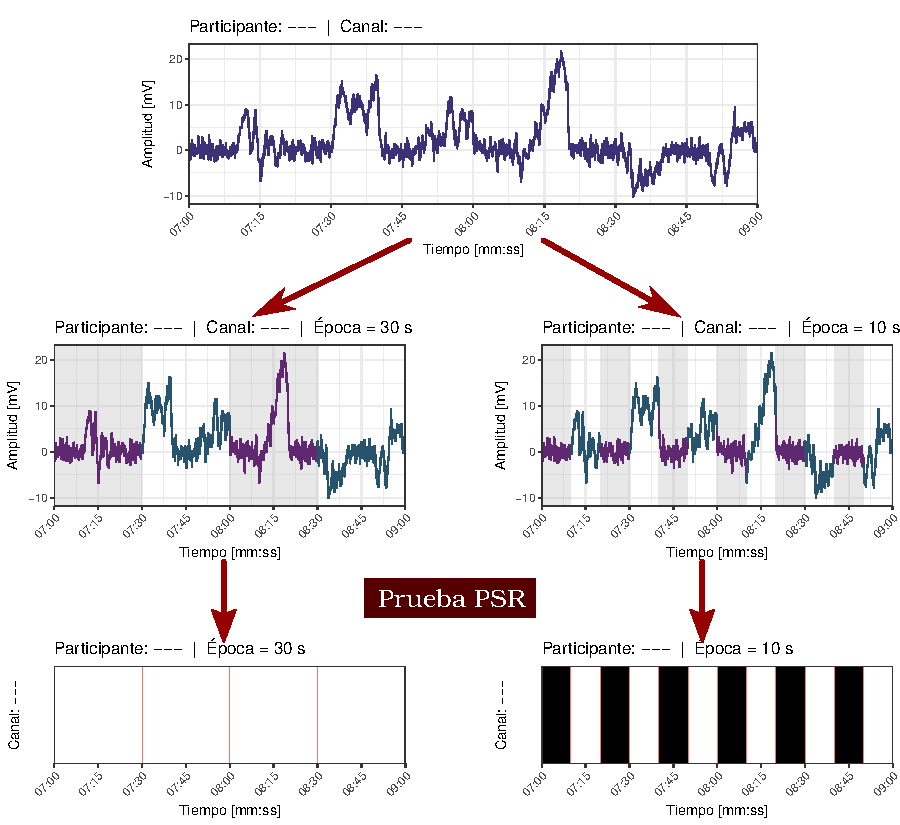
\includegraphics[width=\linewidth]{./img_diagramas/epocas_diferentes_v3.pdf}
\caption{Efecto del tamaño de ventana sobre la clasificación de estacionariedad.}
\label{epocas_diferentes}
\end{figure}

%%%%%%%%%%%%%%%%%%%%%%%%%%%%%%%%%%%%%%%%%%%%%%%%%%%%%%%%%%%%%%%%%%%%%%%%%%%%%%%%%%%%%%%%%%%%%%%%%%%
%%%%%%%%%%%%%%%%%%%%%%%%%%%%%%%%%%%%%%%%%%%%%%%%%%%%%%%%%%%%%%%%%%%%%%%%%%%%%%%%%%%%%%%%%%%%%%%%%%%
%%%%%%%%%%%%%%%%%%%%%%%%%%%%%%%%%%%%%%%%%%%%%%%%%%%%%%%%%%%%%%%%%%%%%%%%%%%%%%%%%%%%%%%%%%%%%%%%%%%
%%%%%%%%%%%%%%%%%%%%%%%%%%%%%%%%%%%%%%%%%%%%%%%%%%%%%%%%%%%%%%%%%%%%%%%%%%%%%%%%%%%%%%%%%%%%%%%%%%%